% Options for packages loaded elsewhere
\PassOptionsToPackage{unicode,linktoc=all}{hyperref}
\PassOptionsToPackage{hyphens}{url}
\PassOptionsToPackage{dvipsnames,svgnames,x11names}{xcolor}
%
\documentclass[
  a4paper,
]{article}
\usepackage{amsmath,amssymb}
\usepackage{lmodern}
\usepackage{iftex}
\ifPDFTeX
  \usepackage[T1]{fontenc}
  \usepackage[utf8]{inputenc}
  \usepackage{textcomp} % provide euro and other symbols
\else % if luatex or xetex
  \usepackage{unicode-math}
  \defaultfontfeatures{Scale=MatchLowercase}
  \defaultfontfeatures[\rmfamily]{Ligatures=TeX,Scale=1}
\fi
% Use upquote if available, for straight quotes in verbatim environments
\IfFileExists{upquote.sty}{\usepackage{upquote}}{}
\IfFileExists{microtype.sty}{% use microtype if available
  \usepackage[]{microtype}
  \UseMicrotypeSet[protrusion]{basicmath} % disable protrusion for tt fonts
}{}
\makeatletter
\@ifundefined{KOMAClassName}{% if non-KOMA class
  \IfFileExists{parskip.sty}{%
    \usepackage{parskip}
  }{% else
    \setlength{\parindent}{0pt}
    \setlength{\parskip}{6pt plus 2pt minus 1pt}}
}{% if KOMA class
  \KOMAoptions{parskip=half}}
\makeatother
\usepackage{xcolor}
\IfFileExists{xurl.sty}{\usepackage{xurl}}{} % add URL line breaks if available
\IfFileExists{bookmark.sty}{\usepackage{bookmark}}{\usepackage{hyperref}}
\hypersetup{
  pdftitle={Eigenvalues and Eigenvectors---Why are they important?},
  pdfauthor={R (Chandra) Chandrasekhar},
  pdflang={en-GB},
  colorlinks=true,
  linkcolor={DarkOliveGreen},
  filecolor={Purple},
  citecolor={DarkKhaki},
  urlcolor={Maroon},
  pdfcreator={LaTeX via pandoc}}
\urlstyle{same} % disable monospaced font for URLs
\usepackage[margin=25mm]{geometry}
\usepackage{longtable,booktabs,array}
\usepackage{calc} % for calculating minipage widths
% Correct order of tables after \paragraph or \subparagraph
\usepackage{etoolbox}
\makeatletter
\patchcmd\longtable{\par}{\if@noskipsec\mbox{}\fi\par}{}{}
\makeatother
% Allow footnotes in longtable head/foot
\IfFileExists{footnotehyper.sty}{\usepackage{footnotehyper}}{\usepackage{footnote}}
\makesavenoteenv{longtable}
\usepackage{graphicx}
\makeatletter
\def\maxwidth{\ifdim\Gin@nat@width>\linewidth\linewidth\else\Gin@nat@width\fi}
\def\maxheight{\ifdim\Gin@nat@height>\textheight\textheight\else\Gin@nat@height\fi}
\makeatother
% Scale images if necessary, so that they will not overflow the page
% margins by default, and it is still possible to overwrite the defaults
% using explicit options in \includegraphics[width, height, ...]{}
\setkeys{Gin}{width=\maxwidth,height=\maxheight,keepaspectratio}
% Set default figure placement to htbp
\makeatletter
\def\fps@figure{htbp}
\makeatother
\setlength{\emergencystretch}{3em} % prevent overfull lines
\providecommand{\tightlist}{%
  \setlength{\itemsep}{0pt}\setlength{\parskip}{0pt}}
\setcounter{secnumdepth}{-\maxdimen} % remove section numbering
\newlength{\cslhangindent}
\setlength{\cslhangindent}{1.5em}
\newlength{\csllabelwidth}
\setlength{\csllabelwidth}{3em}
\newlength{\cslentryspacingunit} % times entry-spacing
\setlength{\cslentryspacingunit}{\parskip}
\newenvironment{CSLReferences}[2] % #1 hanging-ident, #2 entry spacing
 {% don't indent paragraphs
  \setlength{\parindent}{0pt}
  % turn on hanging indent if param 1 is 1
  \ifodd #1
  \let\oldpar\par
  \def\par{\hangindent=\cslhangindent\oldpar}
  \fi
  % set entry spacing
  \setlength{\parskip}{#2\cslentryspacingunit}
 }%
 {}
\usepackage{calc}
\newcommand{\CSLBlock}[1]{#1\hfill\break}
\newcommand{\CSLLeftMargin}[1]{\parbox[t]{\csllabelwidth}{#1}}
\newcommand{\CSLRightInline}[1]{\parbox[t]{\linewidth - \csllabelwidth}{#1}\break}
\newcommand{\CSLIndent}[1]{\hspace{\cslhangindent}#1}
\ifLuaTeX
\usepackage[bidi=basic]{babel}
\else
\usepackage[bidi=default]{babel}
\fi
\babelprovide[main,import]{british}
% get rid of language-specific shorthands (see #6817):
\let\LanguageShortHands\languageshorthands
\def\languageshorthands#1{}
% $HOME/.pandoc/defaults/latex-header-includes.tex
% Common header includes for both lualatex and xelatex engines.
%
% Preliminaries
%
% \PassOptionsToPackage{rgb,dvipsnames,svgnames}{xcolor}
% \PassOptionsToPackage{main=british}{babel}
\AtBeginEnvironment{quote}{\small}
\AtBeginEnvironment{quotation}{\small}
\AtBeginEnvironment{longtable}{\centering}
%
% Packages that are useful to include
%
\usepackage{graphicx}
\usepackage{subcaption}
\usepackage[inkscapeversion=1]{svg}
\usepackage[defaultlines=4,all]{nowidow}
\usepackage[capitalize,noabbrev]{cleveref}
\usepackage{etoolbox}
\usepackage{fontsize}
\usepackage{newunicodechar}
\usepackage{pdflscape}
\usepackage{fnpct}
\usepackage{parskip}
  \setlength{\parindent}{0pt}
\usepackage[style=american]{csquotes}
% \usepackage{setspace} Use the <fontname-plus.tex> files for setspace
%
% noto-plus.tex
% Font-setting header file for use with Pandoc Markdown
% to generate PDF via LuaLaTeX.
% The main font is Noto Serif.
% Other main fonts are also available in appropriately named file.
\usepackage{fontspec}
\usepackage{setspace}
\setstretch{1.3}
%
\defaultfontfeatures{Ligatures=TeX,Scale=MatchLowercase,Renderer=Node} % at the start always
%
% For English
% See also https://tex.stackexchange.com/questions/574047/lualatex-amsthm-polyglossia-charissil-error
% We use Node as Renderer for the Latin Font and Greek Font and HarfBuzz as renderer ofr Indic fonts.
%
\babelfont{rm}[Script=Latin,Scale=1]{NotoSerif}% Config is at $HOME/texmf/tex/latex/NotoSerif.fontspec
%
\babelfont{sf}[Script=Latin]{SourceSansPro}% Config is at $HOME/texmf/tex/latex/SourceSansPro.fontspec
%
\babelfont{tt}[Script=Latin]{FiraMono}% Config is at $HOME/texmf/tex/latex/FiraMono.fontspec
%
% Sanskrit, Tamil, and Greek fonts
%
\babelprovide[import, onchar=ids fonts]{sanskrit}
\babelprovide[import, onchar=ids fonts]{tamil}
\babelprovide[import, onchar=ids fonts]{greek}
%
\babelfont[sanskrit]{rm}[Scale=1.1,Renderer=HarfBuzz,Script=Devanagari]{NotoSerifDevanagari}
\babelfont[sanskrit]{sf}[Scale=1.1,Renderer=HarfBuzz,Script=Devanagari]{NotoSansDevanagari}
\babelfont[tamil]{rm}[Renderer=HarfBuzz,Script=Tamil]{NotoSerifTamil}
\babelfont[tamil]{sf}[Renderer=HarfBuzz,Script=Tamil]{NotoSansTamil}
\babelfont[greek]{rm}[Script=Greek]{GentiumBookPlus}
%
% Math font
%
\usepackage{unicode-math} % seems not to hurt % fallabck
\setmathfont[bold-style=TeX]{STIX Two Math}
%
%
% Other fonts
%
\newfontfamily{\emojifont}{Symbola}
%

\usepackage{titling}
\usepackage{fancyhdr}
    \pagestyle{fancy}
    \fancyhead{}
    \fancyfoot{}
    \renewcommand{\headrulewidth}{0.2pt}
    \renewcommand{\footrulewidth}{0.2pt}
    \fancyhead[LO,RE]{\scshape\thetitle}
    \fancyfoot[CO,CE]{\footnotesize Copyright © 2006\textendash\the\year, R (Chandra) Chandrasekhar}
    \fancyfoot[RE,RO]{\thepage}
\newfontfamily{\regulariconfont}{Font Awesome 6 Free Regular}[Color=Grey]
\newfontfamily{\solidiconfont}{Font Awesome 6 Free Solid}[Color=Grey]
\newfontfamily{\brandsiconfont}{Font Awesome 6 Brands}[Color=Grey]
%
% Direct input of Unicode code points
%
\newcommand{\faEnvelope}{\regulariconfont\ ^^^^f0e0\normalfont}
\newcommand{\faMobile}{\solidiconfont\ ^^^^f3cd\normalfont}
\newcommand{\faLinkedin}{\brandsiconfont\ ^^^^f0e1\normalfont}
\newcommand{\faGithub}{\brandsiconfont\ ^^^^f09b\normalfont}
\newcommand{\faAtom}{\solidiconfont\ ^^^^f5d2\normalfont}
\newcommand{\faPaperPlaneRegular}{\regulariconfont\ ^^^^f1d8\normalfont}
\newcommand{\faPaperPlaneSolid}{\solidiconfont\ ^^^^f1d8\normalfont}

%
% The block below is commented out because of Tofu glyphs in HTML
%
% \newcommand{\faEnvelope}{\regulariconfont\ \normalfont}
% \newcommand{\faMobile}{\solidiconfont\ \normalfont}
% \newcommand{\faLinkedin}{\brandsiconfont\ \normalfont}
% \newcommand{\faGithub}{\brandsiconfont\ \normalfont}
\ifLuaTeX
  \usepackage{selnolig}  % disable illegal ligatures
\fi

\title{Eigenvalues and Eigenvectors---Why are they important?}
\author{R (Chandra) Chandrasekhar}
\date{2015-12-13 | 2020-12-01}

\begin{document}
\maketitle

\thispagestyle{empty}


\hypertarget{stimulating-interest-in-an-arcane-topic}{%
\subsection{Stimulating interest in an arcane
topic}\label{stimulating-interest-in-an-arcane-topic}}

A university academic friend of mine recently remarked that it was not
easy to motivate students to study
\href{https://en.wikipedia.org/wiki/Eigenvalues_and_eigenvectors}{eigenvalues
and eigenvectors,} let alone appreciate their importance: the subject
itself was abstract, and the applications tended to be domain-specific
and somewhat arcane.

A cursory Web search turned up results that confirmed his assertions and
concerns. There have been
\href{http://matheducators.stackexchange.com/questions/520/what-is-a-good-motivation-showcase-for-a-student-for-the-study-of-eigenvalues}{pro}
and
\href{http://matheducators.stackexchange.com/questions/8586/too-much-motivation}{con}
views about motivating students to learn about eigenvalues and
eigenvectors, and especially to convey
\href{http://matheducators.stackexchange.com/questions/3983/what-is-the-best-way-to-intuitively-explain-what-eigenvectors-and-eigenvalues-ar}{intuitively}
their
\href{http://math.stackexchange.com/questions/23312/what-is-the-importance-of-eigenvalues-eigenvectors}{importance}.

I then asked, ``Can I explain to \emph{myself} what eigenvalues and
eigenvectors are, and why they are important?''. It also occurred to me
that the harried and hurried students of today might derive some benefit
from my efforts; hence this blog. It is a brief, largely qualitative,
and mathematically non-rigorous article on eigenvalues and eigenvectors
that aims to provide meaning and motivation for their study. Corrections
and suggestions for improvement are most welcome. \emojifont {🙂}
\normalfont

\hypertarget{eigenvalues-and-eigenvectors}{%
\subsection{Eigenvalues and
eigenvectors}\label{eigenvalues-and-eigenvectors}}

As a general rule, the more powerful an idea, the more prevalent it
becomes. Think about words and numbers, and you will see what I mean.

Eigenvalues and eigenvectors are one such powerful idea. It is no
surprise that they appear in different guises in different contexts: in
oscillating electronic circuits, in dynamical systems, in computer
games, in the spectra of atoms, and in Google searches, to name just a
few.

The word
\href{https://en.wikipedia.org/wiki/Talk:Eigenvector}{\emph{eigen}} is
German in origin and means ``inherent, characteristic, natural, own, or
peculiar (to)''. So the prefix ``eigen'' captures the natural essence of
the noun it qualifies. Perhaps the word ``idiosyncratic'' comes closest
to conveying its import.

\hypertarget{matrices}{%
\subsection{Matrices}\label{matrices}}

Eigenvalues and eigenvectors are associated traditionally with
\href{https://en.wikipedia.org/wiki/Matrix_\%28mathematics\%29}{\emph{matrices}}.
If numbers are like tea-leaves, matrices are like tea-bags. They are
rectangular arrays of numbers, whether real or complex, that have been
hijacked by mathematicians to serve as a shorthand in a variety of
contexts. What they mean depends on context and level of abstraction.
They can represent geometric transformations in Euclidean space, or
systems of linear equations, or systems of linear differential equations
with constant coefficients, or linear transformations in vector spaces.
Note the recurrence of the word \emph{linear} here.

\hypertarget{invariance-and-identity-elements}{%
\subsection{Invariance and identity
elements}\label{invariance-and-identity-elements}}

\href{http://mathworld.wolfram.com/Invariant.html}{Invariance} is a
central concept in mathematics and physics. Adding zero to a number
leaves it unchanged. Multiplying a number by one again leaves it
unchanged. And zero and one are important numbers, usually called the
\emph{additive} and \emph{multiplicative identity elements}
respectively. Consider now the matrix equivalent of multiplying by
\(1\), an example of which is:
\begin{equation}\protect\hypertarget{eq:identity}{}{
\begin{bmatrix}1 & 0\\0 & 1\end{bmatrix}\begin{bmatrix}v_{1}\\v_{2}\end{bmatrix}
= 1\begin{bmatrix}v_{1}\\v_{2}\end{bmatrix} = \begin{bmatrix}v_{1}\\v_{2}\end{bmatrix}
}\label{eq:identity}\end{equation}

The \(2 \times 2\) matrix on the extreme left of \cref{eq:identity} is
the \emph{identity matrix} of dimension \(2\), analogous to the
multiplicative identity. We could write this equation more succinctly
as: \begin{equation}\protect\hypertarget{eq:succinct}{}{
I\symbf{v} = 1\symbf{v}
}\label{eq:succinct}\end{equation} \(I\), on the left, is the
\emph{identity matrix}, the number \(1\) on the right is called an
\emph{eigenvalue} and the vector \(\symbf{v}\) is called an
\emph{eigenvector}. Note that there are no strictures on \(\symbf{v}\).
So, in this particular case, \emph{all} vectors \(\symbf{v}\) are
eigenvectors but there is only \emph{one} eigenvalue, namely \(1\). This
example, however, is both unusual and contrived, because the identity
matrix is a \emph{special} type of \emph{square matrix} with ones on its
principal diagonal and zeros elsewhere.

\cref{eq:succinct} is a particular case of the general equation for
eigenvalues and eigenvectors, which is written:
\begin{equation}\protect\hypertarget{eq:eigen}{}{
M\symbf{v} = \lambda \symbf{v}
}\label{eq:eigen}\end{equation} where \(M\) is a \emph{general square
matrix}, \({\lambda}\) is a \emph{real or complex scalar} called an
\emph{eigenvalue}, and \(\symbf{v}\) is a \emph{non-zero vector} called
an \emph{eigenvector}. The matrix \(M\) is assigned meaning according to
context. Geometrically, the \emph{orientation} of the vector
\(\symbf{v}\) is unchanged by the transformation \(M\), although if
\(\lambda\) is negative, the direction is reversed. Specifically, the
eigenvector corresponding to an eigenvalue of \(1\) remains unchanged by
the transformation---an example of invariance.

\hypertarget{calculus}{%
\subsection{Calculus}\label{calculus}}

The operation of taking a derivative may be denoted by the
\emph{differential operator,} \(D\). We know that \[
\frac{d}{dt}e^{t} = D(e^{t}) = e^{t}
\] and further that \[
\frac{d}{dt}e^{st} = D(e^{st}) = se^{st}
\] where \(s\) is a scalar and \(t\) is the independent variable,
usually time. Although \(D\) is not a matrix here, it is nevertheless a
linear transformation that operates on \emph{functions.} And in place of
a vector, we have a function, \(e^{st}\), which is therefore called an
\emph{eigenfunction} of the differential operator, with eigenvalue
\(s\). The importance of the complex exponentials in signal and system
analysis cannot be over-emphasized: just recall the
\href{https://en.wikipedia.org/wiki/Laplace_transform}{Laplace} and
\href{https://en.wikipedia.org/wiki/Fourier_transform}{Fourier}
transforms.

\hypertarget{differential-equations}{%
\subsection{Differential Equations}\label{differential-equations}}

Linear homogeneous \emph{differential equations} with constant
coefficients may be written using the \(D\) notation already introduced.
A second order homogeneous equation with independent variable \(t\) and
dependent variable \(y\) may be written as
\(a_2D^2(y) + a_1D(y) + a_0(y) = 0\). Plugging in a solution of the form
\(y = e^{st}\), we get \((a_2s^2 + a_1s + a_0)e^{st} = 0.\) Since
\(e^{st}\) can never be zero, we may divide by it to get the
\emph{characteristic polynomial}
\begin{equation}\protect\hypertarget{eq:cp}{}{
a_2s^2 + a_1s + a_0 = 0.
}\label{eq:cp}\end{equation}

The \emph{roots} of this characteristic polynomial give us the
eigenvalues of the system. Perhaps, the prefix ``eigen'' came to be used
because of the adjective ``characteristic''.

These ideas masquerade under different terminology in linear system and
control theory where
\href{https://en.wikipedia.org/wiki/Transfer_function}{transfer
function},
\href{http://web.mit.edu/2.14/www/Handouts/PoleZero.pdf}{poles and
zeros}, \href{https://www.youtube.com/watch?v=hcXbyS2Cf2o}{natural
frequency and resonance}, and
\href{https://en.wikibooks.org/wiki/Control_Systems/Stability}{stability}
are encountered.

\hypertarget{characteristic-polynomial-of-a-square-matrix}{%
\subsection{Characteristic polynomial of a square
matrix}\label{characteristic-polynomial-of-a-square-matrix}}

The characteristic polynomial of a square matrix is obtained likewise.
The equation \(M\symbf{v} = \lambda \symbf{v}\) may be re-written as
\((M -\lambda I)\symbf{v}=\symbf{0}\), where the right hand side is the
\emph{zero vector}. Since the eigenvector \(\symbf{v}\) is non-zero,
this implies that the matrix \((M -\lambda I)\) is
\href{https://en.wikipedia.org/wiki/Invertible_matrix}{singular} or
non-invertible, which in turn implies that its
\href{https://en.wikipedia.org/wiki/Determinant}{determinant} is zero.
So, the characteristic polynomial is the equation
\begin{equation}\protect\hypertarget{eq:cp-matrix}{}{\det(M - \lambda I) = 0
}\label{eq:cp-matrix}\end{equation} and its roots are the eigenvalues of
\(M\). The determinant of a square matrix is a \emph{number} associated
with it, obtained by adding and subtracting products of its elements in
a specific order.

\hypertarget{linear-transformations-and-vector-spaces}{%
\subsection{Linear transformations and vector
spaces}\label{linear-transformations-and-vector-spaces}}

A \href{https://en.wikipedia.org/wiki/Vector_space}{vector space} is a
powerful mathematical abstraction that allows us to unify many disparate
branches of mathematics under a uniform taxonomy.
\href{http://mathworld.wolfram.com/LinearTransformation.html}{Linear
transformations} are a particular type of mapping between two vector
spaces over a scalar field, satisfying:
\begin{equation}\protect\hypertarget{eq:linear}{}{
\begin{aligned}
T(\symbf{u} + \symbf{v}) &= T(\symbf{u}) + T(\symbf{v})\\
T(\alpha\symbf{u}) &= \alpha T(\symbf{u})\\
\end{aligned}
}\label{eq:linear}\end{equation} where \(T\) is the transformation,
\(\symbf{u}\) and \(\symbf{v}\) are two vectors, and \(\alpha\) is a
scalar.

\(T\) may be represented by a matrix, and under certain conditions, its
eigenvalues and eigenvectors can characterize the transformation
\emph{completely.} This happens when (a) all the eigenvectors are
\emph{linearly independent,} i.e., no two eigenvectors are parallel, and
(b) when they \emph{span} the vector space, i.e., any vector within the
space can be constructed from a linear combination of the eigenvectors.
The eigenvectors are then said to form a
\href{https://en.wikipedia.org/wiki/Basis_\%28linear_algebra\%29}{\emph{basis}}
for the space.

As a case in point, let us say \(T\) is a \(3 \times 3\) matrix whose
eigenvectors \(\symbf{e_{1}}\), \(\symbf{e_{2}}\), and \(\symbf{e_{3}}\)
are linearly independent and form a basis. Then, if
\(\symbf{v} = \alpha_{1}\symbf{e_{1}} + \alpha_{2}\symbf{e_{2}} + \alpha_{3}\symbf{e_{3}}\),
where the \(\alpha_{i}\)s are scalars, by virtue of the fact that \(T\)
is a linear transformation, we have \[
\begin{aligned}
T(\symbf{v}) & = T(\alpha_{1}\symbf{e_{1}} + \alpha_{2}\symbf{e_{2}} + \alpha_{3}\symbf{e_{3}})\\
& = T(\alpha_{1}\symbf{e_{1}}) + T(\alpha_{2}\symbf{e_{2}}) + T(\alpha_{3}\symbf{e_{3}})\\
& = \alpha_{1}T(\symbf{e_{1}}) + \alpha_{2}T(\symbf{e_{2}}) + \alpha_{3}T(\symbf{e_{3}})\\
& = \alpha_{1}\lambda{_1}\symbf{e_{1}} + \alpha_{2}\lambda_{2}\symbf{e_{2}} + \alpha_{3}\lambda_{3}\symbf{e_{3}}
\end{aligned}
\] Notice how the right hand side is now expressed \emph{purely as a sum
of scaled eigenvectors.} This is the essence of why eigenvalues and
eigenvectors are so important: they are \emph{sufficient} to describe
what is taking place. \emph{Eigenvalues and eigenvectors encode the
transformation succinctly, just as DNA encodes biological information.}

If, in addition, \(T\) is
\href{https://en.wikipedia.org/wiki/Symmetry_in_mathematics}{\emph{symmetric}},
its eigenvectors form an
\href{https://en.wikipedia.org/wiki/Orthonormality}{\emph{orthonormal
basis}}. Such basis vectors confer \emph{parsimony} (think low
bandwidth) when images or audio signals need to be deconstructed for
transmission and reconstructed on reception. Eigenvectors are also
useful in techniques like
\href{https://en.wikipedia.org/wiki/Principal_component_analysis}{\emph{principal
component analysis}} which is used in statistical pattern recognition.

The applications of eigenvalues and eigenvectors in linear algebra run
far and deep. Suffice it here to merely mention that an extension,
fortuitously called
\href{https://en.wikipedia.org/wiki/Spectral_theory}{\emph{spectral
theory,}} even explains the observed spectra of atoms in quantum theory!

\hypertarget{a-property-of-eigenvectors}{%
\subsubsection{A property of
eigenvectors}\label{a-property-of-eigenvectors}}

I will here belabour a point that might seem blindingly obvious to some
but frustratingly obscure to others. Let \(\symbf{v}\) be an eigenvector
associated with a distinct eigenvalue \(\lambda\) as in \cref{eq:eigen},
and let \(k\) be a non-zero scalar. Then, using the second of the
equation-pair \cref{eq:linear}, we have
\begin{equation}\protect\hypertarget{eq:scaled-eigenvector}{}{
M(k\symbf{v}) = k(M\symbf{v}) = k(\lambda\symbf{v}) = \lambda(k\symbf{v}),
}\label{eq:scaled-eigenvector}\end{equation} which means that if
\(\symbf{v}\) is an eigenvector, any non-zero scalar multiple of
\(\symbf{v}\) is also an eigenvector for that same eigenvalue. So,
strictly speaking, we really should be referring to \emph{an}
eigenvector---rather than \emph{the} eigenevctor---corresponding to any
given eigenvalue.

\hypertarget{worked-example}{%
\subsection{Worked example}\label{worked-example}}

A worked example would normally have made its way here at this point in
the article. But because the example is long and might not interest
everyone, I have relegated it to the end of the article. Stay tuned if
you are enthused.

\hypertarget{resources}{%
\subsection{Resources}\label{resources}}

I hope that this article has not been so brief as to be cryptic and
off-putting. To those in search of greater rigour or a more formal
exposition, I would recommend a good linear algebra textbook. The
venerable tome that I used at university went by the acronym ``KKOP''
after the initials of the surnames of the four authors, Kreider, Kuller,
Ostberg, and Perkins {[}\protect\hyperlink{ref-kkop1966}{1}{]}.
Unfortunately, it is out of print, but as a consolation, \cref{fig:kkop}
is an image of my copy. \emojifont {😞}\normalfont

\begin{figure}
\hypertarget{fig:kkop}{%
\centering
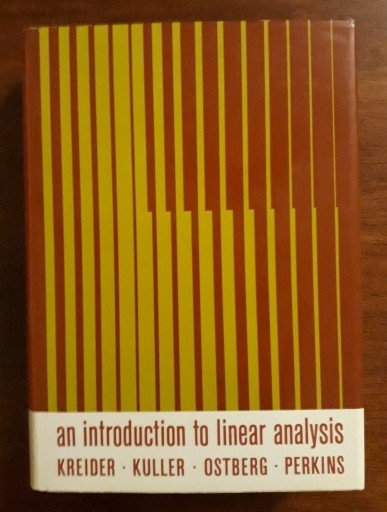
\includegraphics[width=0.5\textwidth,height=\textheight]{images/kkop.jpg}
\caption{The KKOP book: \emph{An Introduction to Linear
Analysis}.}\label{fig:kkop}
}
\end{figure}

For something more contemporary, I would recommend the textbooks and
lectures of Professor Gilbert Strang of MIT. They are attuned to those
who \emph{apply} mathematics, like engineers and scientists. There is an
\href{https://archive.org/details/MIT18.06S05_MP4}{archived video of his
lecture on eigenvalues and eigenvectors.} There are also links to
\href{http://ocw.mit.edu/courses/mathematics/18-06-linear-algebra-spring-2010/}{his
MIT Open Course Ware (OCW) page for Course 18.06 of Spring 2010},
\href{http://math.mit.edu/~gs/linearalgebra/}{his linear algebra
textbook home page} {[}\protect\hyperlink{ref-strang2016}{2}{]}, and
\href{http://www-math.mit.edu/~gs/}{his academic home page.}

Many academics make their lecture notes freely available online:
\href{https://www.google.com/}{google} for them.
\href{https://www.youtube.com/}{You Tube} videos of lectures are another
source of information and knowledge, which offer the immediacy of a
classroom lecture with the convenience of instant rewind in case you
need to catch something you missed.

Online forums offer a slightly more interactive learning experience but
again, their depth and quality varies. The
\href{http://math.stackexchange.com/}{Mathematics StackExchange} and
\href{https://www.quora.com/}{Quora} are two sites that you might
explore.

Examples of all the above types of resources have been tucked away
within the various links in this article: try them out to get a flavour
of what is available.

\hypertarget{importance-and-applications}{%
\subsection{Importance and
applications}\label{importance-and-applications}}

If, after all this, you are still unconvinced about the utility of
eigenvalues and eigenvectors, think of this analogy. Crystals have
natural
\href{https://en.wikipedia.org/wiki/Cleavage_\%28crystal\%29}{\emph{cleavage
planes}} that allow them to be fractured easily along specific
directions. This exploits the \emph{symmetry} in the crystals. Likewise,
eigenvalues and eigenvectors exploit the naturally occurring symmetries
of mathematical structures and transformations to allow us to view them
more simply and insightfully. Without eigenvalues and eigenvectors, we
would have neither radios nor lasers.

To get an idea of the broad sweep of eigenvalues and their
applicability, I strongly recommend that you should read a charming
article entitled
\href{http://people.maths.ox.ac.uk/trefethen/dec11.pdf}{``Favourite
Eigenvalue Problems''.} Another article that takes a breezy look at the
subject of this writeup is
\href{http://hubpages.com/education/What-the-Heck-are-Eigenvalues-and-Eigenvectors}{``What
the Heck are Eigenvalues and Eigenvectors?''.} It has a disputed
explanation (see comments on the article) of how a bridge collapsed---so
take that
\href{https://www.thefreedictionary.com/cum+grano+salis}{\emph{cum grano
salis}}. It also contains a link to a PDF paper interestingly entitled
\href{http://www.rose-hulman.edu/~bryan/googleFinalVersionFixed.pdf}{``The
25,000,000,000.00 Dollar Eigenvector: The Linear Algebra Behind
Google'',} which, in good faith, I think is not a spoof! Indeed, the
\href{http://ilpubs.stanford.edu:8090/422/}{citation to the original
Stanford InfoLab technical report} and the
\href{http://ilpubs.stanford.edu:8090/422/1/1999-66.pdf}{actual report}
are both available online.

\hypertarget{worked-example-modelling-weather-with-a-transition-matrix}{%
\subsection{Worked example: modelling weather with a transition
matrix}\label{worked-example-modelling-weather-with-a-transition-matrix}}

Now for the promised example of eigenvalues at work---in a simplified
real-life situation, modelling the weather. Let us assume that
yesterday's weather influences the \emph{probability} of today's
weather, and today's weather influences the \emph{probability} of
tomorrow's weather. Each day's weather depends only on the previous
day's weather, i.e., the weather has a ``memory'' of one day.

To keep it simple, let us have only three weather states: sunny, cloudy,
and rainy, with the stipulation that each day can only be \emph{one} of
these three. Further, in our matrix, let the ordering be sunny, cloudy,
and rainy, both left to right, and top to bottom. Then, the column
headings represent \emph{today's weather} and the row headings represent
\emph{tomorrow's weather.} We then have the
\href{https://en.wikipedia.org/wiki/Stochastic_matrix}{\emph{state-transition
matrix}} or \emph{Markov matrix} \(M\) given in \cref{eq:state}:
\begin{equation}\protect\hypertarget{eq:state}{}{
M = \begin{bmatrix}
0.65 & 0.30 & 0.10\\
0.25 & 0.45 & 0.40\\
0.10 & 0.25 & 0.50
\end{bmatrix}
}\label{eq:state}\end{equation}

Note that each \emph{column} of \(M\) represents the probabilities of
\href{https://en.wikipedia.org/wiki/Mutual_exclusivity}{\emph{mutually
exclusive}} events, which must therefore sum to one. The matrix element
\(m_{ij}\) is the probability that today's weather is in column \(j\)
and that tomorrow's weather is in row \(i\). For example, The
probability of today being rainy and tomorrow cloudy is given by
\(m_{23} = 0.40\).

Let the column-vector \(\symbf{w}_{k}\) represent the probabilities for
a particular day's weather and the column-vector \(\symbf{ w}_{k+1}\),
the next day's weather. The two are then related by:
\begin{equation}\protect\hypertarget{eq:recurrence}{}{
\symbf{w}_{k+1} = M\symbf{w}_{k}
}\label{eq:recurrence}\end{equation} \cref{eq:recurrence}) is called a
\href{https://en.wikipedia.org/wiki/Recurrence_relation}{\emph{recurrence
relation}} or \emph{difference equation}, and in our case, it represents
the evolution of a dynamical system in time, namely the weather. Just
for completeness, let the initial condition be given by:
\begin{equation}\protect\hypertarget{eq:initial}{}{
\symbf{w}_{0} = \begin{bmatrix}0.55\\0.34\\0.11\end{bmatrix}
}\label{eq:initial}\end{equation}

We want to know whether, for this model, there will be an equilibrium or
steady-state in the weather, represented by a probability vector with
values that remain steady with temporal evolution. The question is how
do we find that out?

One obvious way is to compute the downstream weather one day at a time:
think of forging a chain one link at a time because the weather has a
memory of only one day. From \cref{eq:recurrence} we can compute the
following: \[
\begin{aligned}
\symbf{w}_{1} &= M\symbf {w}_{0}\\
&= \begin{bmatrix}0.47050\\ 0.33450\\0.19500\end{bmatrix}\\
\symbf{w}_{2} &= M\symbf{w}_{1}\\
&= M(M\symbf{w}_{0})\\
&= M^{2}\symbf{w}_{0}\\
&= \begin{bmatrix}0.42568\\0.34615\\0.228180\\\end{bmatrix}
\end{aligned}
\]

By induction, the weather vector \(n\) days downstream is given by
\begin{equation}\protect\hypertarget{eq:Mn}{}{
\symbf{w}_{n} = M^{n}\symbf{w}_{0}.
}\label{eq:Mn}\end{equation}

In this manner, we can trace the time evolution of the weather and, if
desired, draw a three-dimensional parametric plot of the successive
weather vectors in \(\mathbb{R}^{3}\) with time as parameter. This could
be insightful, but it is a laborious and time-consuming way to find out
the steady-state weather vector if there is one. Could we do better?

A rough and ready method would be to evaluate \cref{eq:Mn} with \(n\)
set to large numbers, say \(50\) and \(100\), and check if the resulting
weather vectors, \(\symbf{w}_{50}\) and \(\symbf{w}_{100}\) were equal.
If they were, we might hazard a guess that this unchanging value is the
steady-state weather vector.

But computing the fiftieth or one-hunderdth power of a matrix is tedious
and error-prone if done by hand, and computationally expensive if done
by machine, especially if the matrix in question is large.

To devise a better solution, we need to digress briefly to examine
diagonal matrices and the diagonalization of square matrices.

\hypertarget{diagonal-matrix-raised-to-a-power}{%
\subsubsection{Diagonal matrix raised to a
power}\label{diagonal-matrix-raised-to-a-power}}

Suppose that \(D\) is a \(3 \times 3\) diagonal matrix with non-zero
entries on its principal diagonal and zeros elsewhere: \[
D = \begin{bmatrix}
\lambda_{1} & 0 & 0\\
0 & \lambda_{2} & 0\\
0 & 0 & \lambda_{3}
\end{bmatrix}.
\]

Observe that: \begin{equation}\protect\hypertarget{eq:D-to-the-n}{}{
D^{n} = \begin{bmatrix}
\lambda_{1}^{n}& 0 & 0\\
0 & \lambda_{2} ^{n}& 0\\
0 & 0 & \lambda_{3}^{n}
\end{bmatrix}.
}\label{eq:D-to-the-n}\end{equation}

If we could somehow decompose \(M\) into a matrix product where a
diagonal matrix was featured, we might be able to circumvent the
matrix-raised-to-a large-power problem.

\hypertarget{matrix-diagonalization-or-eigen-decomposition}{%
\subsubsection{Matrix diagonalization or eigen
decomposition}\label{matrix-diagonalization-or-eigen-decomposition}}

We need to
\href{http://mathworld.wolfram.com/MatrixDiagonalization.html}{\emph{diagonalize}}
the transition matrix---a procedure called
\href{http://mathworld.wolfram.com/EigenDecomposition.html}{\emph{eigen
decomposition.}} A square matrix with non-repeating eigenvalues and
therefore, linearly independent eigenvectors, can be diagonalized. We
demonstrate how this is done for the \(3 \times 3\) case below.

Let the three eigenvectors be so denoted: \[
\symbf{e}_{k} = \begin{bmatrix}
e_{k1}\\
e_{k2}\\
e_{k3}
\end{bmatrix} ; k = 1, 2, 3.
\] The matrix \(P\) whose \emph{columns} are the eigenvectors is
therefore \[
P = \begin{bmatrix}
e_{11} & e_{21} & e_{31}\\
e_{12} & e_{22} & e_{32}\\
e_{13} & e_{23} & e_{33}
\end{bmatrix}
= \begin{bmatrix}
\symbf{e}_{1} & \symbf{e}_{2} & \symbf{e}_{3}\\
\end{bmatrix}
\] Now, \begin{equation}\protect\hypertarget{eq:diag1}{}{
\begin{aligned}
MP &= M\begin{bmatrix}
\symbf{e}_{1} & \symbf{e}_{2} & \symbf{e}_{3}
\end{bmatrix}\\
&= \begin{bmatrix}
M\symbf{e}_{1} & M\symbf{e}_{2} & M\symbf{e}_{3}
\end{bmatrix}\\
&= \begin{bmatrix}
\lambda_{1}\symbf{e}_{1} & \lambda_{2}\symbf{e}_{2} & \lambda_{3}\symbf{e}_{3}
\end{bmatrix}\\
&= \begin{bmatrix}
e_{11} & e_{21} & e_{31}\\
e_{12} & e_{22} & e_{32}\\
e_{13} & e_{23} & e_{33}
\end{bmatrix}
\begin{bmatrix}
\lambda_{1} & 0 & 0\\
0 & \lambda_{2} & 0\\
0 & 0 & \lambda_{3}
\end{bmatrix}\\
&= PD
\end{aligned}
}\label{eq:diag1}\end{equation} To get only \(M\) on the left-hand side
of \cref{eq:diag1}, we post-multiply both sides by \(P^{-1}\), the
inverse of \(P\):
\begin{equation}\protect\hypertarget{eq:eigendecomp}{}{
MPP^{-1} = MI = M = PDP^{-1}
}\label{eq:eigendecomp}\end{equation} If we now square \(M\), we get
\begin{equation}\protect\hypertarget{eq:D-squared}{}{
\begin{aligned}
M^{2} &= (PDP^{-1})(PDP^{-1})\\
&= PD(P^{-1}P)DP^{-1}\\
&= P(DID)P^{-1}\\
&= PD^{2}P^{-1}
\end{aligned}
}\label{eq:D-squared}\end{equation}

By induction, \begin{equation}\protect\hypertarget{eq:M-to-the-n}{}{
M^{n} = PD^{n}P^{-1}
}\label{eq:M-to-the-n}\end{equation} The role of eigenvalues and
eigenvectors in the plot of raising a square matrix to a power is now
fully revealed: recall that in \cref{eq:M-to-the-n}, \(P\) is the matrix
whose columns are the eigenvectors, and \(D\) is the diagonal matrix
whose non-zero elements are the corresponding eigenvalues, and
\(P^{-1}\) is the inverse of \(P\).

\hypertarget{software-implementation}{%
\subsection{Software Implementation}\label{software-implementation}}

To get numerical results, I initially tried implementing the above steps
with the free open-source mathematics software system
\href{http://www.sagemath.org/}{SageMath,} but found it less than
convenient for my purpose.

I then experimented with \href{https://www.gnu.org/software/octave/}{GNU
Octave,} which is a free, platform-neutral, open source, high-level
interpreted language, primarily intended for numerical computations. It
was better suited to the task at hand, and I easily obtained the results
discussed below.

The self-explanatory file,
\href{auxiliary/weather.m}{\texttt{weather.m}}, may be downloaded and
executed on the command line in the Octave command window. The
discussion below will make better sense after you have thus executed the
file \texttt{weather.m}. Instructions on how to download and set up
Octave are given
\href{https://www.gnu.org/software/octave/download}{here}.

\hypertarget{discussion-of-results-from-weather.m}{%
\subsection{\texorpdfstring{Discussion of results from
\texttt{weather.m}}{Discussion of results from weather.m}}\label{discussion-of-results-from-weather.m}}

The roots of the characteristic polynomial of \(M\) are first evaluated,
and compared to the eigenvalues and eigenvectors obtained from an Octave
function designed for that explicit purpose.

There are \emph{three} distinct eigenvalues for the transition matrix,
\(M\). Moreover,
\href{http://www.math.cornell.edu/~mec/Winter2009/RalucaRemus/Lecture1/lecture1.html}{it
may be proved} that \(1\) is an eigenvalue of any transition matrix. The
eigenvalues we get are: \[
\begin{aligned}
\lambda_{1} &= 1.00000\\
\lambda_{2} &= 0.48028\\
\lambda_{3} &= 0.11972
\end{aligned}
\]

From \cref{eq:M-to-the-n} we may surmise that the contributions from
\(\lambda_{2}\) and \(\lambda_{3}\), being both less than one, will
diminish progressively as \(n\) increases, and in the limit, only the
eigenvalue \(1\) will dominate the steady-state behaviour.

The eigenvectors associated respectively with these eigenvalues, as
spewed out by Octave, are: \[
\symbf{e}_{1} = \begin{bmatrix}
-0.65375\\
-0.61639\\
-0.43895\\
\end{bmatrix}
\quad
\symbf{e}_{2} = \begin{bmatrix}
-0.80430\\
0.28039\\
0.52391\\
\end{bmatrix}
\quad
\symbf{e}_{3} = \begin{bmatrix}
0.37921\\
-0.81582\\
0.43662\\
\end{bmatrix}
\]

None of the column sums of these eigenvectors sums to one. Indeed, the
column sums of \(\symbf{e}_{2}\) and \(\symbf{e}_{3}\) are close to
zero, whereas the column sum of \(\symbf{e}_{1}\) is negative. We will
return to the eigenvector \(\symbf{e}_{1}\), to wrest meaning out of it,
a little later. In any case, we confirm that
\(M\symbf{e}_{1} = \symbf{e}_{1}\).

Assembling the matrices \(P\) and \(P^{-1}\) from the eigenvectors is
trivial, as is putting together \(D\) as the diagonal matrix of the
corresponding eigenvalues. With these numerical values, the truth of
\cref{eq:eigendecomp} is also easily demonstrated.

The time evolution of the initial weather vector is then tracked with 1,
10, 20, 50, and 100 iterations of \cref{eq:recurrence}. In this case,
the weather vector stabilizes after about twenty iterations to a
steady-state vector, \(\symbf{w}_{\infty}\), given by
\begin{equation}\protect\hypertarget{eq:steady-state}{}{
\symbf{w}_{\infty} = \begin{bmatrix}
0.38251\\
0.36066\\
0.25683\\
\end{bmatrix}
}\label{eq:steady-state}\end{equation}

When we track the same temporal evolution for eigenvector
\(\symbf{e}_{1}\), the result after each iteration is \(\symbf{e}_{1}\)
itself. This is the expected behaviour for an eigenvector associated
with an eigenvalue of \(1\).

What may be disconcerting, though, is that we now seem to have
\emph{two} steady-state vectors, \(\symbf{w}_{\infty}\) and
\(\symbf{e}_{1}\).

Observe, however, that \(\symbf{e}_{1}\) is not a probability vector
whose columns sum to one. To convert it to a probability vector, we
\emph{normalize} \(\symbf{e}_{1}\) by dividing it by its column sum, to
get the \emph{normalized eigenvector:}
\begin{equation}\protect\hypertarget{eq:normalized-eigenvector-1}{}{
\symbf{n}_{1} = \begin{bmatrix}
0.38251\\
0.36066\\
0.25683\\
\end{bmatrix}
}\label{eq:normalized-eigenvector-1}\end{equation}

Lo and behold! \(\symbf{n}_{1}\) and \(\symbf{w}_{\infty}\) are one and
the same, and all is well. Recalling from \cref{eq:scaled-eigenvector}
that non-zero scalar multiples of eigenvectors are also eigenvectors
themselves, this result, even if a little magical, really should not
surprise us.

We do not bother normalizing the eigenvectors associated with
\(\lambda_{2}\) and \(\lambda_{3}\) because their column sums almost
vanish, and moreover, their contribution to the steady state decreases
with increasing number of iterations.

To round things off, we substitute a random initial weather vector in
place of \(\symbf{w}_{0}\), and view its evolution over time for twenty
iterations, and find that it too converges to the steady-state weather
vector after about 15 iterations.

This means that regardless of what initial weather vector we start with,
in about two weeks we will end up with a vector that represents the
steady-state.

Observations like these suggest that our inferences are only as good as
our assumptions and models. Oversimplification could lead to absurd
results, and weather prediction over time is a seriously non-trivial
problem.

One general hypothesis that we could examine is whether it is generally
true that the normalized eigenvector associated with an eigenvalue of
\(1\) does indeed represent the steady state of the system represented
by any transition matrix. If so, we would have a theorem on our hands.

\hypertarget{feedback}{%
\subsection{Feedback}\label{feedback}}

Please \href{mailto:feedback.swanlotus@gmail.com}{email me} your
comments and corrections.

\noindent A PDF version of this article is
\href{./eigenvalues-and-eigenvectors.pdf}{available for download here}:

\begin{small}

\begin{sffamily}

\url{https://swanlotus.netlify.app/blogs/eigenvalues-and-eigenvectors.pdf}

\end{sffamily}

\end{small}

\hypertarget{bibliography}{%
\section*{References}\label{bibliography}}
\addcontentsline{toc}{section}{References}

\hypertarget{refs}{}
\begin{CSLReferences}{0}{0}
\leavevmode\vadjust pre{\hypertarget{ref-kkop1966}{}}%
\CSLLeftMargin{1. }%
\CSLRightInline{Kreider, Donald L, Kuller, Robert G, Ostberg, Donald R
and Perkins, Fred W. \emph{{An Introduction to Linear Analysis}}.
Addison-Wesley Publishing Company, 1966. Addison-wesley series in
mathematics. }

\leavevmode\vadjust pre{\hypertarget{ref-strang2016}{}}%
\CSLLeftMargin{2. }%
\CSLRightInline{Strang, Gilbert. \emph{{Introduction to Linear
Algebra}}. 5th ed. Wellesley-Cambridge Press, 2016. }

\end{CSLReferences}



\end{document}
